\documentclass{article}

\usepackage[utf8]{inputenc}
% To remove the line numbers for the camera-ready version of your paper, remove
% the `review` option from the tismir package
\usepackage{tismir}
\usepackage{amsmath}
\usepackage{hyperref}
\usepackage{url}
\usepackage{graphicx}
\usepackage{booktabs}
\usepackage{lipsum}
\usepackage{subcaption} 
\usepackage{tikz}
\usepackage{float}
\usepackage{array} 
\usepackage{multirow}
\usepackage{makecell}
\usetikzlibrary{shapes.geometric, arrows.meta, positioning}


\graphicspath{ {./figures/} }
\urlstyle{same}

%%%%%%%%%%%%%%%%%%%%%%%%%%%%%%%%%%%%%%%%%%%%%%%%%%%%%%%%%%%%%%%%%%%%%%%%%%%%%%%%
% Title and Author information
%%%%%%%%%%%%%%%%%%%%%%%%%%%%%%%%%%%%%%%%%%%%%%%%%%%%%%%%%%%%%%%%%%%%%%%%%%%%%%%%

\title{Power to the People!  Assigning Popular Music Genres Based on Listeners' Perspective Using a Genre Tree Approach}
%

\author{Anonymous}
% \author{%
% Markus Radke\thanks{Audio Communication Group, Technische Universität Berlin, Einsteinufer 17c, 10587 Berlin, Germany} %
% ~and Steffen Lepa\protect\footnotemark[1]}

\date{}

%%%%%%%%%%%%%%%%%%%%%%%%%%%%%%%%%%%%%%%%%%%%%%%%%%%%%%%%%%%%%%%%%%%%%%%%%%%%%%%%
% Additional Paper Information
%%%%%%%%%%%%%%%%%%%%%%%%%%%%%%%%%%%%%%%%%%%%%%%%%%%%%%%%%%%%%%%%%%%%%%%%%%%%%%%%

\type{research}

% Citation in First Page
\authorref{Anonymous}
% \authorref{Radke,~M. and Lepa,~S.}

%
% (Optional)
% \journalyear{2017}
% \journalvolume{V}
% \journalissue{N}
% \journalpages{xx--xx}
% \doi{xx.xxxx/xxxx.xx}

% Remaining Pages (Optional)
\authorshort{Anonymous} 
% \authorshort{Radke, M. and Lepa, S.} 
\titleshort{Power to the People! Assigning Popular Music Genres}
\fancyhead[L]{{}}
\title{Appendix}

\begin{document}
% \maketitle

\huge\sf\textbf{Appendix}
\normalsize
\appendix
\renewcommand\thefigure{\thesection.\arabic{figure}}    
\renewcommand\thetable{\thesection.\arabic{table}}    
\setcounter{figure}{0} 
\section{Detailed FOLDCAT flowchart for folding COMGET to identify genre categories}
\vspace{0.5cm}

\noindent\makebox[\textwidth][l]{%
  \hspace*{-0.9cm}%
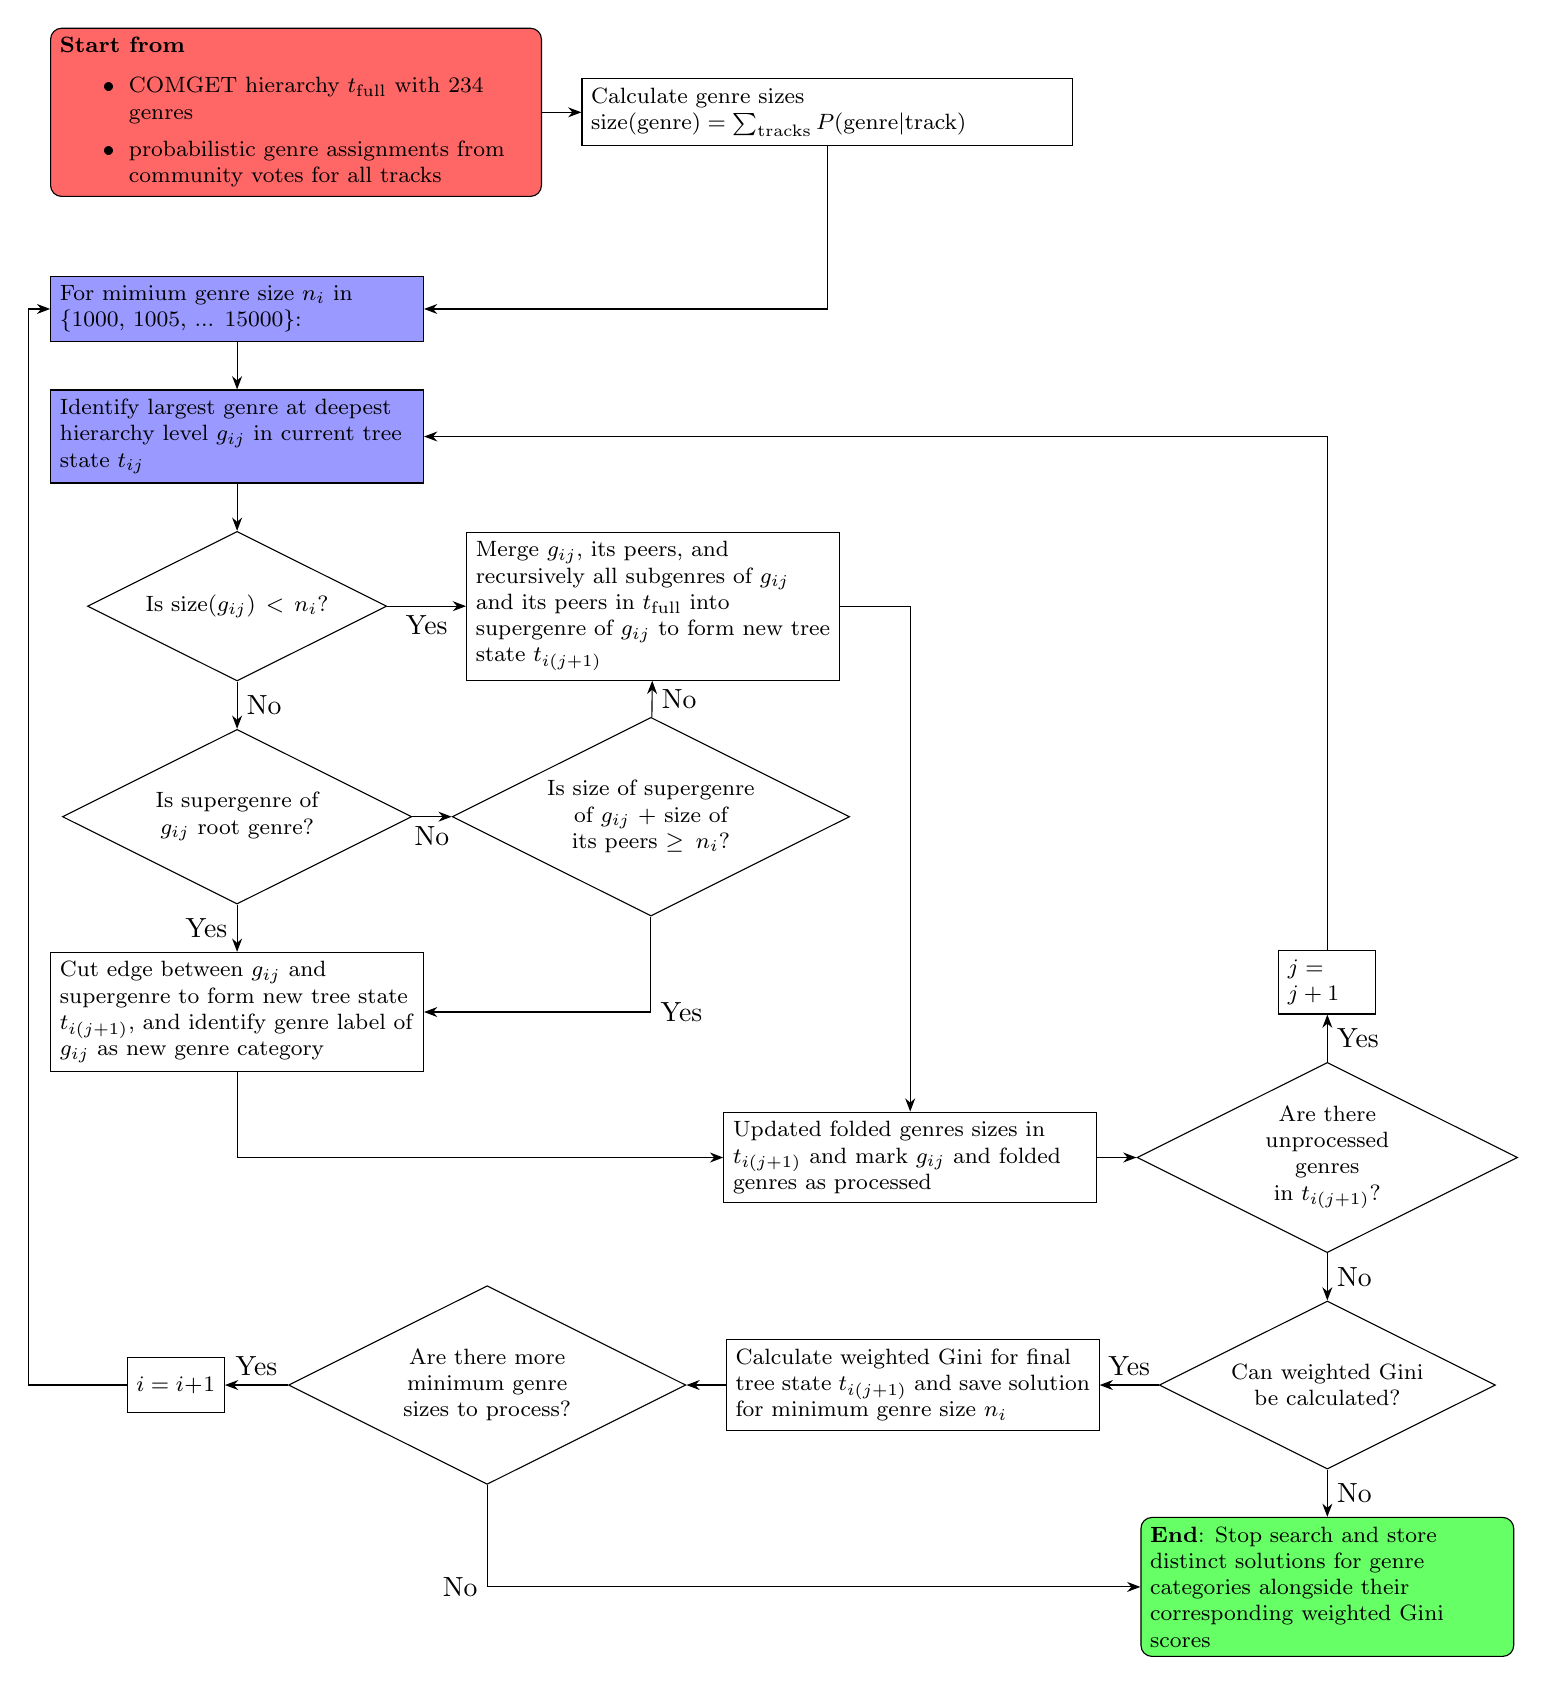
\begin{tikzpicture}[
    node distance=6mm and 5mm,
    terminator/.style = {rectangle, draw, align=flush left, text width = 4.5cm, rounded corners, minimum height=2em, font = \footnotesize},
    process/.style = {rectangle, draw, align=flush left, text width = 4.5cm, minimum height=2em, font = \footnotesize},
    decision/.style = {diamond, draw, aspect=2, text centered, inner sep=1pt, text width = 3 cm, minimum height=2em, font = \footnotesize},
    >=Stealth]

\node[terminator, text width = 6 cm, fill=red!60] (A) {
  \textbf{Start from}\\
    \begin{itemize}
      \item COMGET hierarchy $t_{\text{full}}$ with 234 genres
      \item probabilistic genre assignments from community votes for all tracks
    \end{itemize}
  };
  \node[process, right=of A, text width = 6cm] (B) {Calculate genre sizes \\$\text{size(genre)}=\sum_{\text{tracks}} P(\text{genre}|\text{track})$};
  \node[process, below left=10mm and -47.5mm of A, fill=blue!40] (C) {For mimium genre size $n_i$ in \{1000, 1005, ... 15000\}:};
  \node[process, below=of C, fill=blue!40] (D) {Identify largest genre at deepest hierarchy level $g_{ij}$ in current tree  state $t_{ij}$};
  \node[decision, below=of D] (E) {Is $\text{size}(g_{ij}) < n_i$?};
  \node[process, right=10mm of E] (F) {Merge $g_{ij}$, its peers, and recursively all subgenres of $g_{ij}$ and its peers in $t_{\text{full}}$ into supergenre of $g_{ij}$ to form new tree state $t_{i(j+1)}$};
  \node[decision, below=of E] (G) {Is supergenre of $g_{ij}$ root genre?};
  \node[decision, right=of G] (H) {Is size of supergenre of $g_{ij}$ + size of its peers $\geq n_i$?};
  \node[process, below=of G] (I) {Cut edge between $g_{ij}$ and supergenre to form new tree state $t_{i(j+1)}$, and identify genre label of $g_{ij}$ as new genre category};
  \node[process, below right=5mm and 38 mm of I] (J) {Updated folded genres sizes in $t_{i(j+1)}$ and mark $g_{ij}$ and folded genres as processed};
  \node[decision, text width = 2cm, right=5mm of J] (K) {Are there\\unprocessed\\genres\\in $t_{i(j+1)}$?};
  \node[process, text width = 1cm, above=of K] (L) {$j = j + 1$};
  \node[decision, below=of K] (M) {Can weighted Gini be calculated?};
  \node[terminator, below=of M, fill=green!60] (N) {\textbf{End}: Stop search and store distinct solutions for genre categories alongside their corresponding weighted Gini scores}; 
  \node[process, left=7.5mm of M] (O) {Calculate weighted Gini for final tree state $t_{i(j+1)}$ and save solution for minimum genre size $n_i$};  
  \node[decision, left=of O] (P) {Are there more minimum genre sizes to process?};
  \node[process, text width = 1cm, left=8mm of P] (Q) {$i = i + 1$};




  %connectors
  \draw[->] (A) -- (B);
  \draw[->] (B) |- (C);
  \draw[->] (C) -- (D);
  \draw[->] (D) -- (E);
  \draw[->] (E) -- node[anchor=north] {Yes} (F);
  \draw[->] (E) -- node[anchor=west] {No} (G);
  \draw[->] (G) -- node[anchor=north] {No} (H);
  \draw[->] (H) -- node[anchor=west] {No} (F);
  \draw[->] (H) |- node[anchor=west] {Yes} (I);
  \draw[->] (G) -- node[anchor=east] {Yes} (I);
  \draw[->] (I) |- (J);
  \draw[->] (F) -| (J);
  \draw[->] (J) -- (K);
  \draw[->] (K) -- node[anchor=west] {Yes} (L);
  \draw[->] (L) |- (D);
  \draw[->] (K) -- node[anchor=west] {No} (M);
  \draw[->] (M) -- node[anchor=west] {No} (N);
  \draw[->] (M) -- node[anchor=south] {Yes} (O);
  \draw[->] (O) -- (P);
  \draw[->] (P) -- node[anchor=south] {Yes} (Q);
  \draw [->] 
    (Q.west) -- +(-1.25,0) |-  (C);
  \draw[->] (P) |- node[anchor=east] {No} (N);
\end{tikzpicture}
}

\newpage
\section{RQ3 Machine Learning Workflow}
\subsection*{Overall Workflow}
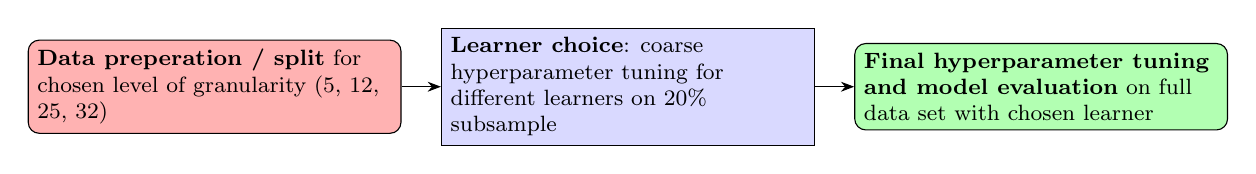
\begin{tikzpicture}[
    node distance=6mm and 5mm,
    terminator/.style = {rectangle, draw, align=flush left, text width = 4.5cm, rounded corners, minimum height=2em, font = \footnotesize},
    process/.style = {rectangle, draw, align=flush left, text width = 4.5cm, minimum height=2em, font = \footnotesize},
    decision/.style = {diamond, draw, aspect=2, text centered, inner sep=1pt, text width = 3 cm, minimum height=2em, font = \footnotesize},
    >=Stealth]

    \node[terminator, fill=red!30] (A) {\textbf{Data preperation / split} for chosen level of granularity (5, 12, 25, 32)};
    \node[process, right=of A, fill=blue!15] (B) {\textbf{Learner choice}: coarse hyperparameter tuning for different learners on 20\% subsample};
    \node[terminator, fill=green!30, right=of B] (C) {\textbf{Final hyperparameter tuning and model evaluation} on full data set with chosen learner};

    \draw[->] (A) -- (B);
    \draw[->] (B) -- (C);
\end{tikzpicture}

\vspace{1 cm}
\subsection{Data preperation / split}
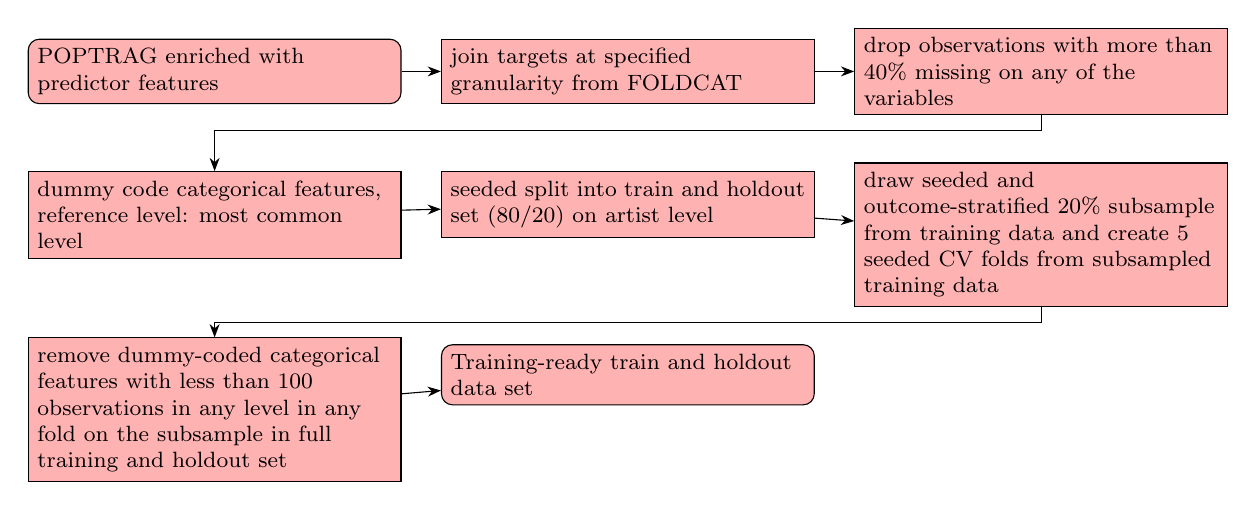
\begin{tikzpicture}[
    node distance=6mm and 5mm,
    terminator/.style = {rectangle, draw, align=flush left, text width = 4.5cm, rounded corners, minimum height=2em, font = \footnotesize, fill=red!30},
    process/.style = {rectangle, draw, align=flush left, text width = 4.5cm, minimum height=2em, font = \footnotesize, fill=red!30},
    >=Stealth]

    \node[terminator] (A) {POPTRAG enriched with predictor features};
    \node[process, right=of A] (B) {join targets at specified granularity from FOLDCAT};
    \node[process, right=of B] (C) {drop observations with more than 40\% missing on any of the variables};
    \node[process, below=8.5mm of A] (D) {dummy code categorical features, reference level: most common level};
    \node[process, below=8.5mm of B] (E) {seeded split into train and holdout set (80/20) on artist level};
    \node[process, below=of C] (F) {draw seeded and outcome-stratified 20\% subsample from training data and create 5 seeded CV folds from subsampled training data};
    \node[process, below=10 mmof D] (G) {remove dummy-coded categorical features with less than 100 observations in any level in any fold on the subsample in full training and holdout set};
    \node[terminator, below=13.5mm of E] (H) {Training-ready train and holdout data set};
    
    \draw[->] (A) -- (B);
    \draw[->] (B) -- (C);
    \draw[->] (C.south) --+ (0,-0.2) -| (D);
    \draw[->] (D) -- (E);
    \draw[->] (E) -- (F);
    \draw[->] (F.south) --+ (0,-0.2) -| (G);
    \draw[->] (G) -- (H);
\end{tikzpicture}

\vspace{1 cm}
\subsection{Learner Choice}
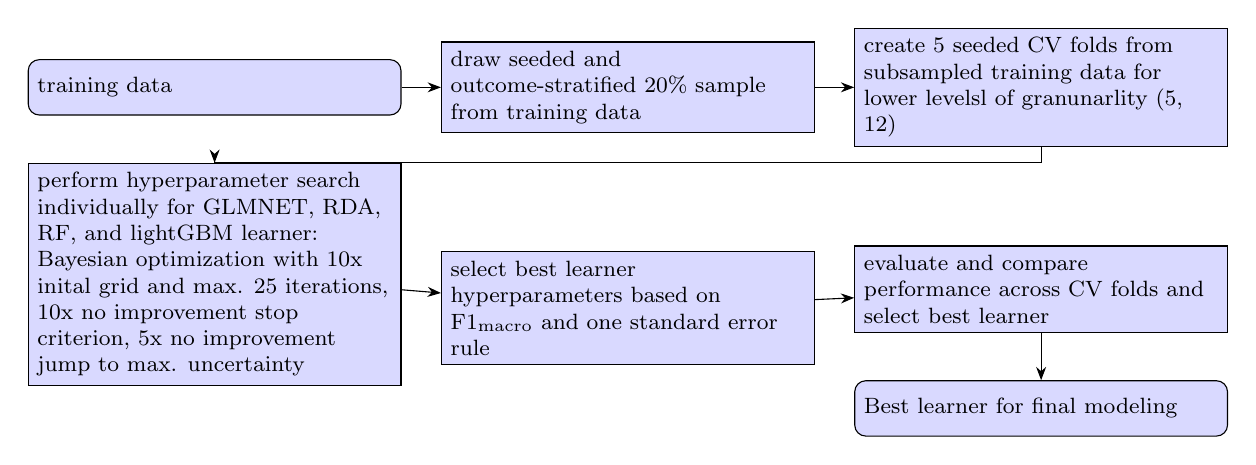
\begin{tikzpicture}[
    node distance=6mm and 5mm,
    terminator/.style = {rectangle, draw, align=flush left, text width = 4.5cm, rounded corners, minimum height=2em, font = \footnotesize, fill=blue!15},
    process/.style = {rectangle, draw, align=flush left, text width = 4.5cm, minimum height=2em, font = \footnotesize, fill=blue!15},
    >=Stealth]

    \node[terminator] (A) {training data};
    \node[process, right=of A] (B) {draw seeded and outcome-stratified 20\% sample from training data};
    \node[process, right=of B] (C) {create 5 seeded CV folds from subsampled training data for lower levelsl of granunarlity (5, 12)};
    \node[process, below=of A] (D) {perform hyperparameter search individually for GLMNET, RDA, RF, and lightGBM learner: Bayesian optimization with 10x inital grid and max. 25 iterations, 10x no improvement stop criterion, 5x no improvement jump to max. uncertainty};
    \node[process, below=15mm of B] (E) {select best learner hyperparameters based on $\text{F1}_{\text{macro}}$ and one standard error rule};
    \node[process, below=12.5mm of C] (F) {evaluate and compare performance across CV folds and select best learner};
    \node[terminator, below=of F] (G) {Best learner for final modeling};

    \draw[->] (A) -- (B);
    \draw[->] (B) -- (C);
    \draw[->] (C.south) --+ (0, -0.2) -| (D);
    \draw[->] (D) -- (E);
    \draw[->] (E) -- (F);
    \draw[->] (F) -- (G);
    
\end{tikzpicture}

\vspace{1 cm}
\subsection{Final Hyperparameter tuning and model evaluation}
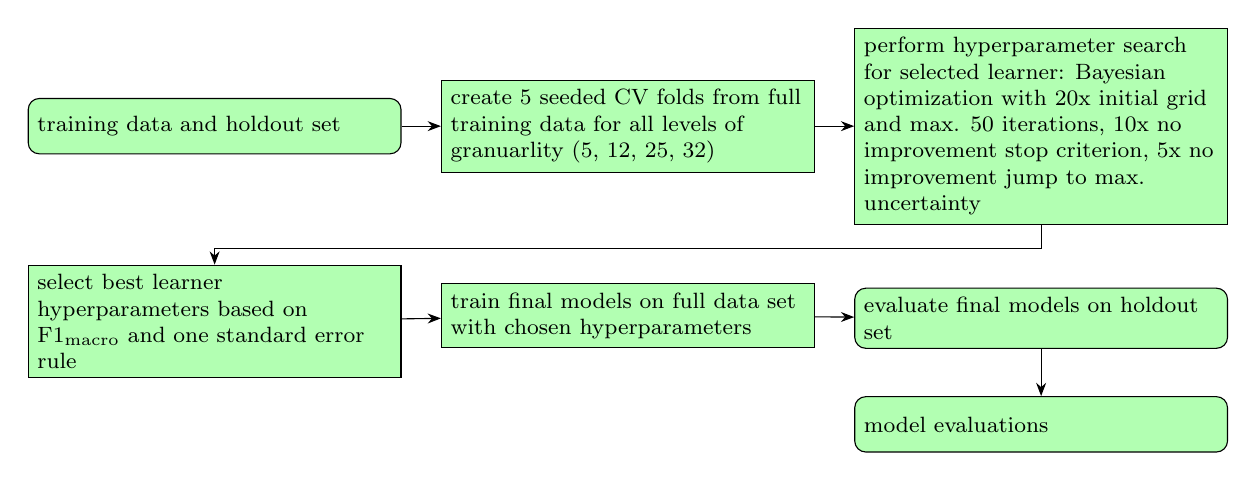
\begin{tikzpicture}[
    node distance=6mm and 5mm,
    terminator/.style = {rectangle, draw, align=flush left, text width = 4.5cm, rounded corners, minimum height=2em, font = \footnotesize, fill=green!30},
    process/.style = {rectangle, draw, align=flush left, text width = 4.5cm, minimum height=2em, font = \footnotesize, fill=green!30},
    >=Stealth]

    \node[terminator] (A) {training data and holdout set};
    \node[process, right=of A] (B) {create 5 seeded CV folds from full training data for all levels of granuarlity (5, 12, 25, 32)};
    \node[process, right=of B] (C) {perform hyperparameter search for selected learner: Bayesian optimization with 20x initial grid and max. 50 iterations, 10x no improvement stop criterion, 5x no improvement jump to max. uncertainty};
    \node[process, below=14 mmof A] (D) {select best learner hyperparameters based on $\text{F1}_{\text{macro}}$ and one standard error rule};
    \node[process, below=14 mmof B] (E) {train final models on full data set with chosen hyperparameters};
    \node[terminator, below=8mm of C] (F) {evaluate final models on holdout set};
    \node[terminator, below=of F] (G) {model evaluations};

    \draw[->] (A) -- (B);
    \draw[->] (B) -- (C);
    \draw[->] (C.south) --+ (0, -0.3) -| (D);
    \draw[->] (D) -- (E);
    \draw[->] (E) -- (F);
    \draw[->] (F) -- (G);
\end{tikzpicture}

\newpage
\subsection{Data preprocessing recipe during training and evalutation}

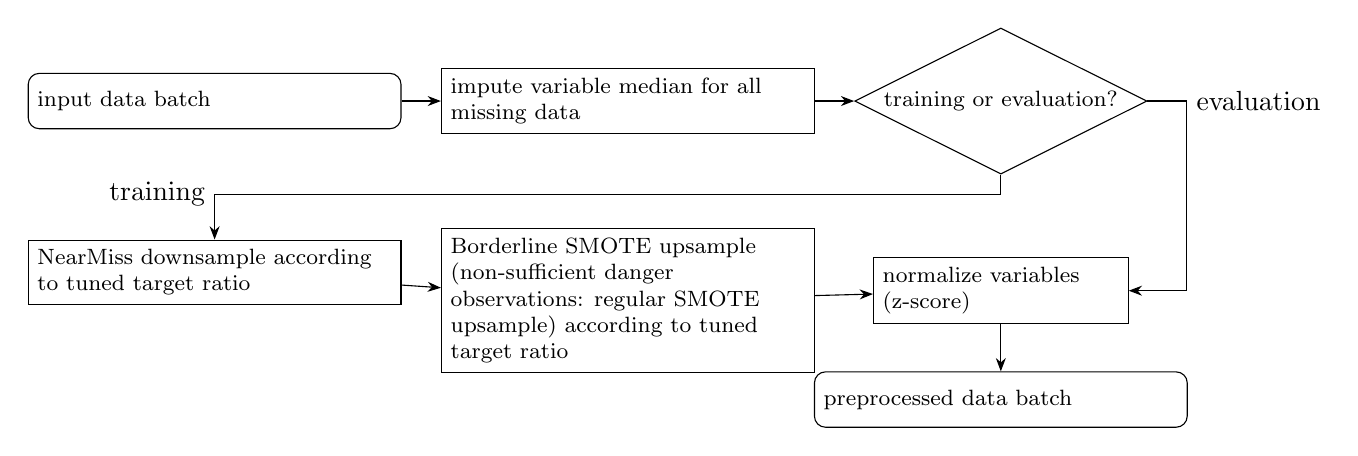
\begin{tikzpicture}[
    node distance=6mm and 5mm,
    terminator/.style = {rectangle, draw, align=flush left, text width = 4.5cm, rounded corners, minimum height=2em, font = \footnotesize},
    process/.style = {rectangle, draw, align=flush left, text width = 4.5cm, minimum height=2em, font = \footnotesize},
    decision/.style = {diamond, draw, aspect=2, text centered, inner sep=1pt, text width = 3 cm, minimum height=2em, font = \footnotesize},
    >=Stealth]

    \node[terminator] (A) {input data batch};
    \node[process, right=of A] (B) {impute variable median for all missing data};
    \node[decision, right=of B] (C) {training or evaluation? };
    \node[process, below=14mm of A] (D) {NearMiss downsample according to tuned target ratio};
    \node[process, below=12mm of B] (E) {Borderline SMOTE upsample (non-sufficient danger observations: regular SMOTE upsample) according to tuned target ratio};
    \node[process, below=10.5mm of C, text width=3 cm] (F) {normalize variables (z-score)};
    \node[terminator, below=of F] (G) {preprocessed data batch}; 
    

    \draw[->] (A) -- (B);
    \draw[->] (B) -- (C);
    \draw[->] (C.east) --+ (0.5, 0) node[anchor=west] {evaluation} |- (F);
    \draw[->] (C.south) --+  (0, -0.25)  -|  node[anchor=east] {training} (D);
    \draw[->] (D) -- (E);
    \draw[->] (E) -- (F);
    \draw[->] (F) -- (G);
\end{tikzpicture}

\newpage
\section{RQ3 features}
\begin{table}[!h]
  \centering
  \footnotesize
  \label{tab:features_for_classification}
  \begin{tabular}{>{\raggedright\arraybackslash}p{0.1\linewidth}|>{\raggedright\arraybackslash}p{0.1667\linewidth}|>{\raggedright\arraybackslash}p{0.1667\linewidth}|>{\raggedright\arraybackslash}p{0.12\linewidth}|>{\raggedright\arraybackslash}p{0.1667\linewidth}|>{\raggedright\arraybackslash}p{0.1667\linewidth}}
\toprule
\multicolumn{1}{c}{\textbf{Construct}} &
\multicolumn{1}{c}{\textbf{Subdimensions}} &
\multicolumn{1}{c}{\textbf{Data Type}} &
\multicolumn{1}{c}{\textbf{Indicators}} &
\multicolumn{1}{c}{\textbf{Variable Content}} &
\multicolumn{1}{c}{\textbf{Source}} \\ \midrule
    \multirow{51}{*}{\makecell[l]{genre of a\\popular\\music track}} & \multirow{15}{*}{\makecell[l]{release milieu\\(via metadata)}} & \multirow{11}{*}{metadata release} & \multirow{7}{*}{artist} & gender & \multirow{6}{*}{\textit{MusicBrainz}} \\ 
     &  &  &  & persona &  \\
     &  &  &  & country of activity &  \\
     &  &  &  & country of origin &  \\
     &  &  &  & birth year &  \\
     &  &  &  & is dead?  &  \\ \cline{6-6}
     &  &  &  & 27 Spotify distribution genres & \textit{Spotify} \\ \cline{4-6}
     &  &  & \multirow{4}{*}{release} & release year & \multirow{4}{*}{\makecell[l]{\textit{MusicBrainz}\\ \textit{Spotify}}}\\
     &  &  &  & indie label?  & \\
     &  &  &  & D-A-CH label?  &  \\
     &  &  &  & release length &  \\ \cline{3-6}
     &  & \multirow{4}{*}{metadata lyrics} & \multirow{2}{*}{code system} & language & \textit{Genius / MusicBrainz} \\ \cline{6-6}
     &  &  &  & track explicit?  & \textit{Spotify} \\  \cline{4-6}
     &  &  & \multirow{2}{*}{\makecell[l]{information\\content}} & distinct words ratio & \multirow{2}{*}{\textit{Genius}} \\
     &  &  &  & repeated lines ratio &  \\ \cline{2-6}
     & \multirow{29}{*}{\makecell[l]{musical style\\(via content analysis)}} & \multirow{10}{*}{\makecell[l]{lexial content analysis\\of lyrics}} & \multirow{10}{*}{emotion} & positive & \multirow{10}{*}{\textit{Genius + syuzhet}} \\
     &  &  &  & negative &  \\
     &  &  &  & anger &  \\
     &  &  &  & disgust &  \\
     &  &  &  & fear &  \\
     &  &  &  & joy &  \\
     &  &  &  & sadness &  \\
     &  &  &  & suprise &  \\
     &  &  &  & anticipation &  \\
     &  &  &  & trust &  \\ \cline{4-6}
     &  &  & topics & sentiment & \textit{Genius + sentimentr} \\ \cline{3-6}
     &  & \multirow{19}{*}{\makecell[l]{machine-learning-\\based audio signal\\analysis}} & \multirow{5}{*}{\makecell[l]{sound of\\production}} & loudness & \multirow{19}{*}{\makecell[l]{\textit{Spotify} (\textit{Echo-Nest})\\\textit{Acousticbrainz}\\(\textit{Essentia})}} \\
     &  &  &  & brightness &  \\
     &  &  &  & acousticness &  \\
     &  &  &  & liveness &  \\
     &  &  &  & typicality genre sounds &  \\ \cline{4-5}
     &  &  & \multirow{4}{*}{instrumnetation} & instrumentalness &  \\
     &  &  &  & tonality &  \\
     &  &  &  & voice and female voice sound &  \\
     &  &  &  & electronic sound &  \\ \cline{4-5}
     &  &  & \multirow{9}{*}{composition} & tempo &  \\
     &  &  &  & chords structure &  \\
     &  &  &  & duration &  \\
     &  &  &  & time signature &  \\
     &  &  &  & key &  \\
     &  &  &  & rhythm &  \\
     &  &  &  & danceability &  \\
     &  &  &  & emotional expression &  \\
     &  &  &  & mood &  \\ \cline{2-6}
     & \multirow{8}{*}{\makecell[l]{popularity\\(via sucess metrics)}} & \multirow{8}{*}{\makecell[l]{streams, followers, and\\release numbers\\on commercial music\\streaming platforms}} & \multirow{2}{*}{track} & popularity & \textit{Spotify} \\ \cline{6-6}
     &  &  &  & rank & \textit{Deezer} \\ \cline{4-6}
     &  &  & \multirow{3}{*}{artist} & streams & \textit{Spotify} \\ \cline{6-6}
     &  &  &  & followers & \multirow{2}{*}{\textit{Deezer}}\\ 
     &  &  &  & number of releases &  \\ \cline{4-6}
     &  &  & \multirow{3}{*}{label} & median track populariy & \multirow{3}{*}{\textit{Spotify}} \\
     &  &  &  & median release popularity &  \\
     &  &  &  & median track popularity &  \\ \bottomrule
  \end{tabular}
  \caption{Features used for training the automated classifier and their theoretical dimension, adapted from 
  % \citep{lepaRadke2026}
  anonymous autors (XXXX).}
\end{table}


\newpage
\normalsize
\section{RQ3 classification hyperparmeters and outcomes for higher granularities}

\begin{figure}[H]
    \centering
    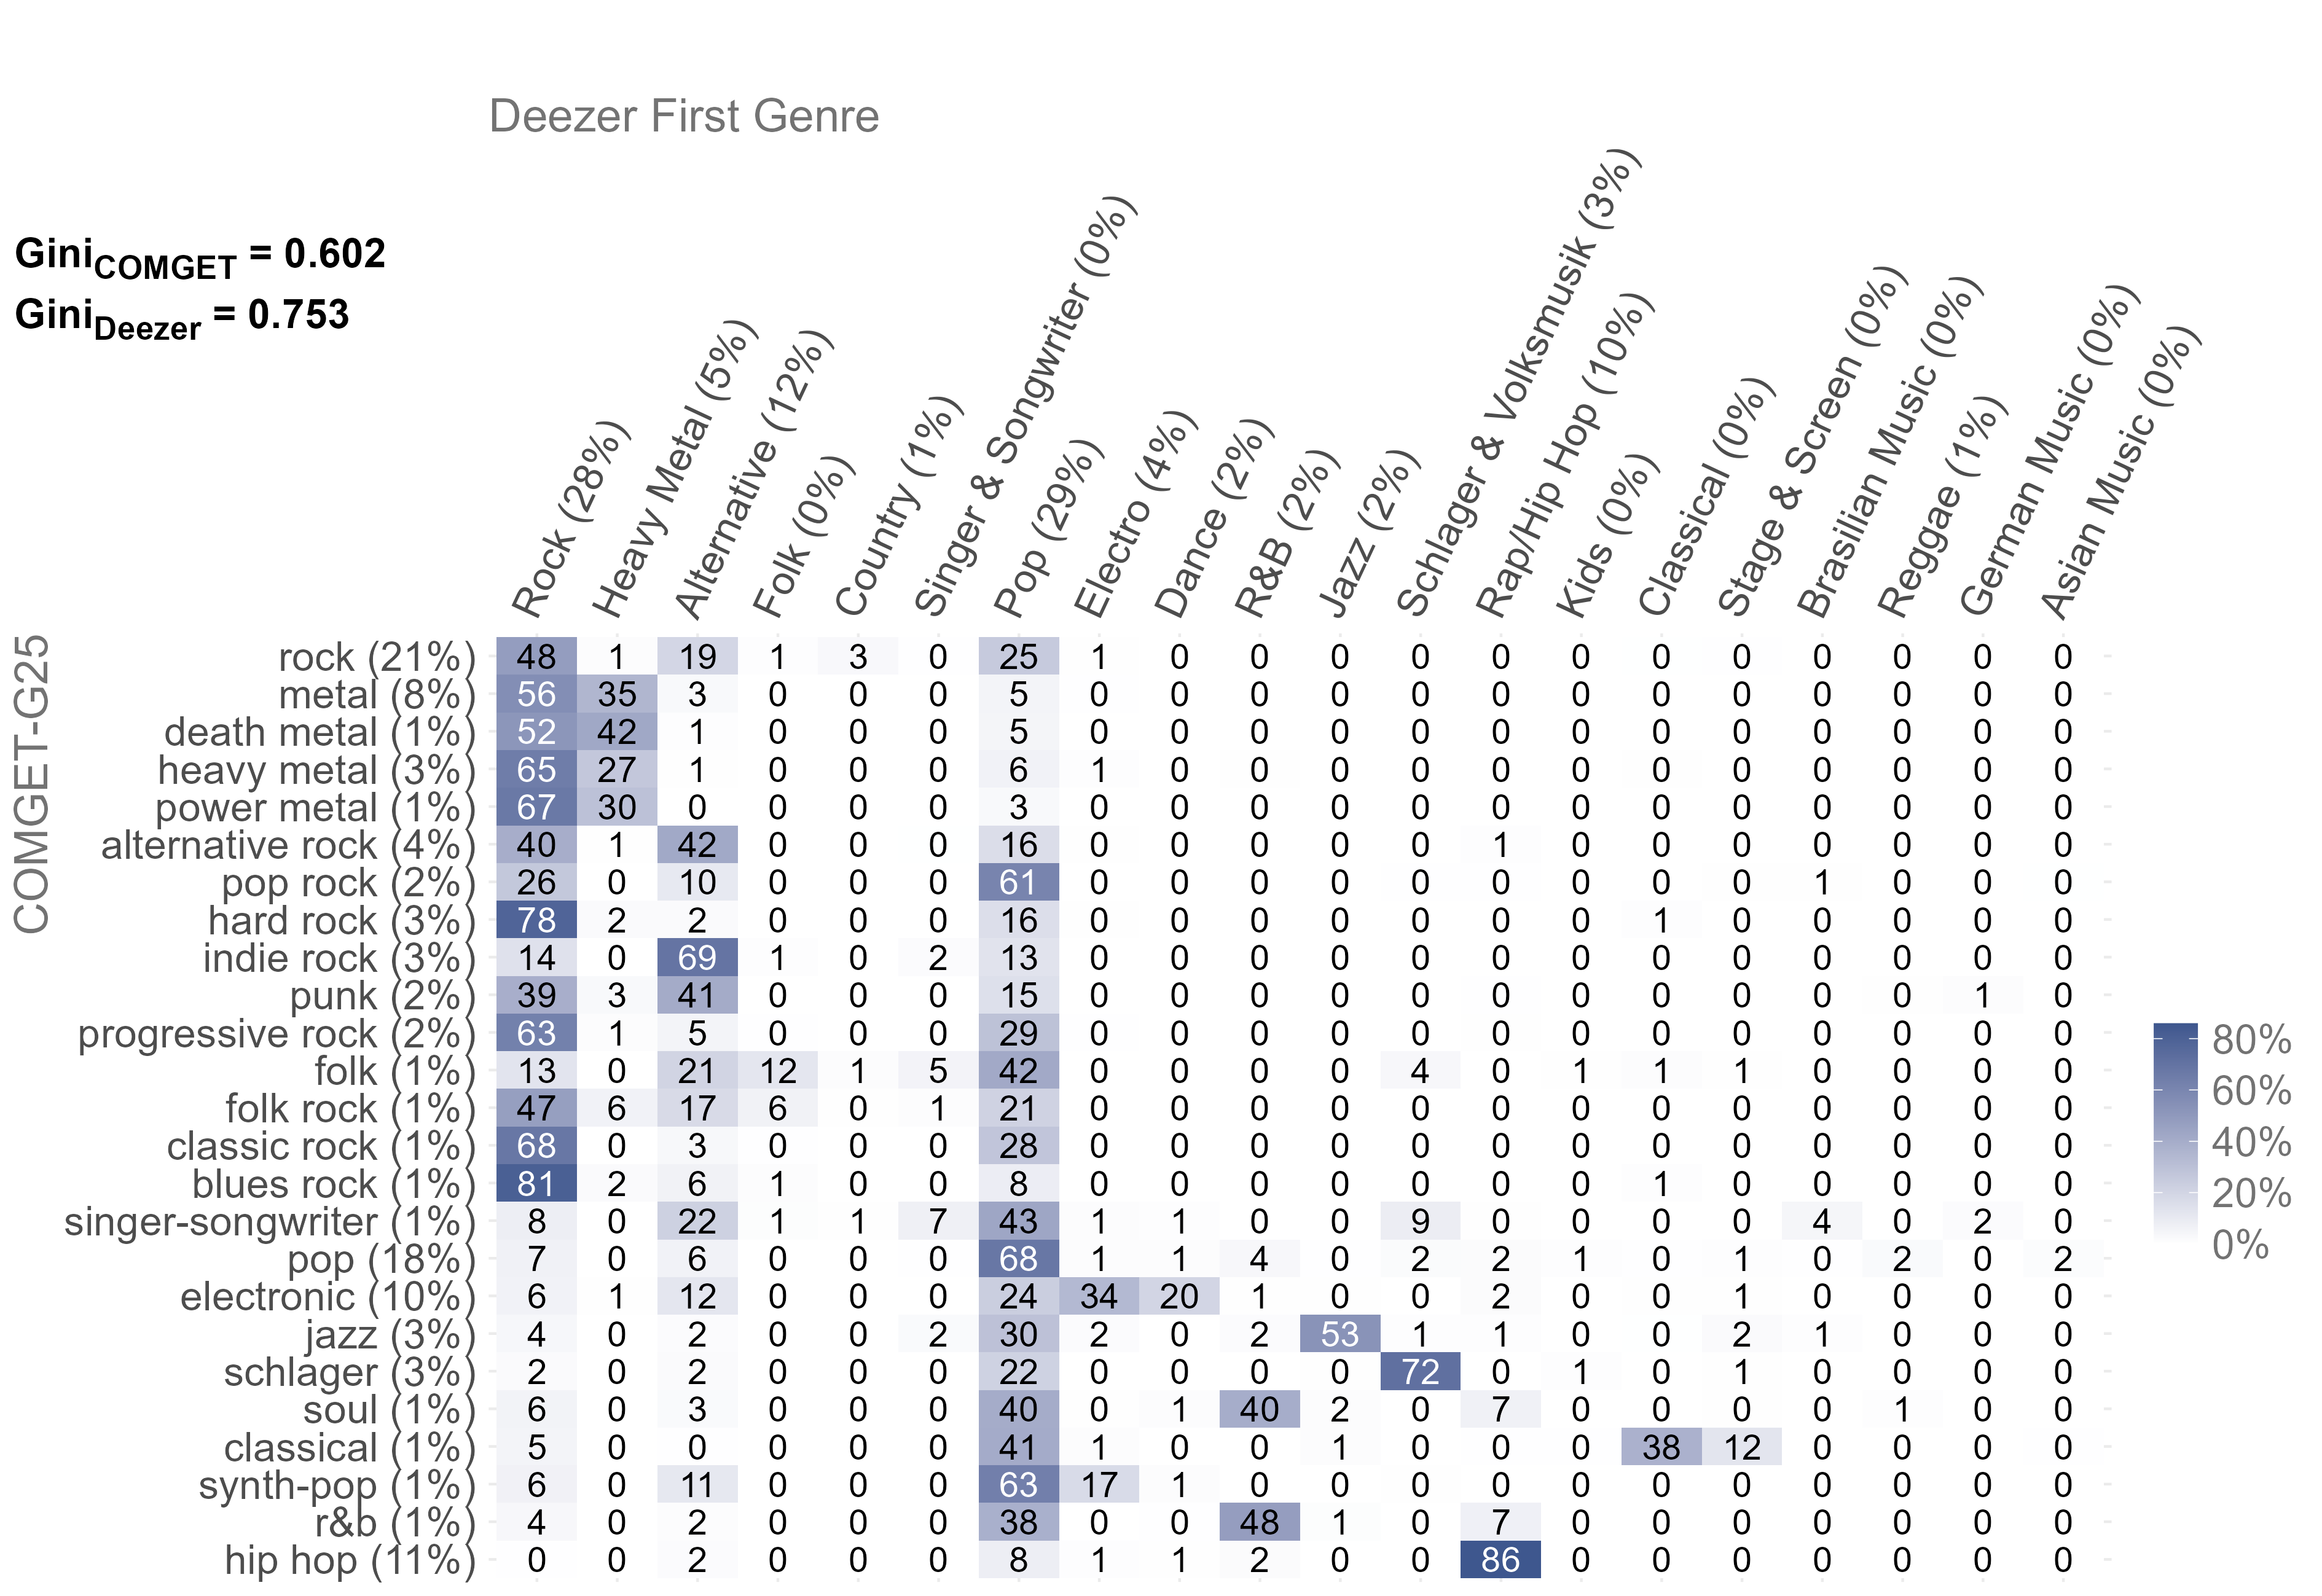
\includegraphics[width=\linewidth]{figures/dz_contingency.png}
    \caption{Contingency tables comparing COMGET-G25 to release genres from the \textit{Deezer} API; 27 genres were found in the data set; values show $P(\text{COMGET} \mid \text{External})$. Discarded 15 genres for visualization with less than 0.5\% relative freuqency: \textit{African Music, Asian Music, Bolero, Brasilian Music, Classical, Disco, Film / Video Games, Folk, German Music, Kids, Latin Music, Ranchera, Singer \& Songwriter, Soul \& Funk, Turkish Folk Music}.}
    \label{fig:placeholder}
\end{figure}


\vspace{2 cm}
\setcounter{table}{0} 
\begin{table*}[htbp]
\centering
\begin{tabular}{lllllll}
\# genres & boosting rounds & tree depth & feature fraction & leaf size & learning rate & target ratio \\
& [50, 2000] & [3, 15] & [1, \# of predictors] & [1, 100] & [0.001, 0.1] & [1, max/min] \\
\hline
5 & 93 & 12 & 68 & 46 & 0.072 & 4.815 \\
12 & 1145 & 10 & 5 & 28 & 0.046 & 2.116\\
25 & 1512 & 9 & 85 & 91 & 0.005 & 2.641\\ 
32 & 176 & 9 & 55 & 15 & 0.0182 & 4.589
\end{tabular}
\caption{Hyperparameter settings for final LightGBM models at different granularity levels.}
\label{tab:rq3_hyperparams}
\end{table*}
\newpage    

\begin{figure}[H]
  \centering
  \begin{subfigure}[b]{\textwidth}
    \centering
    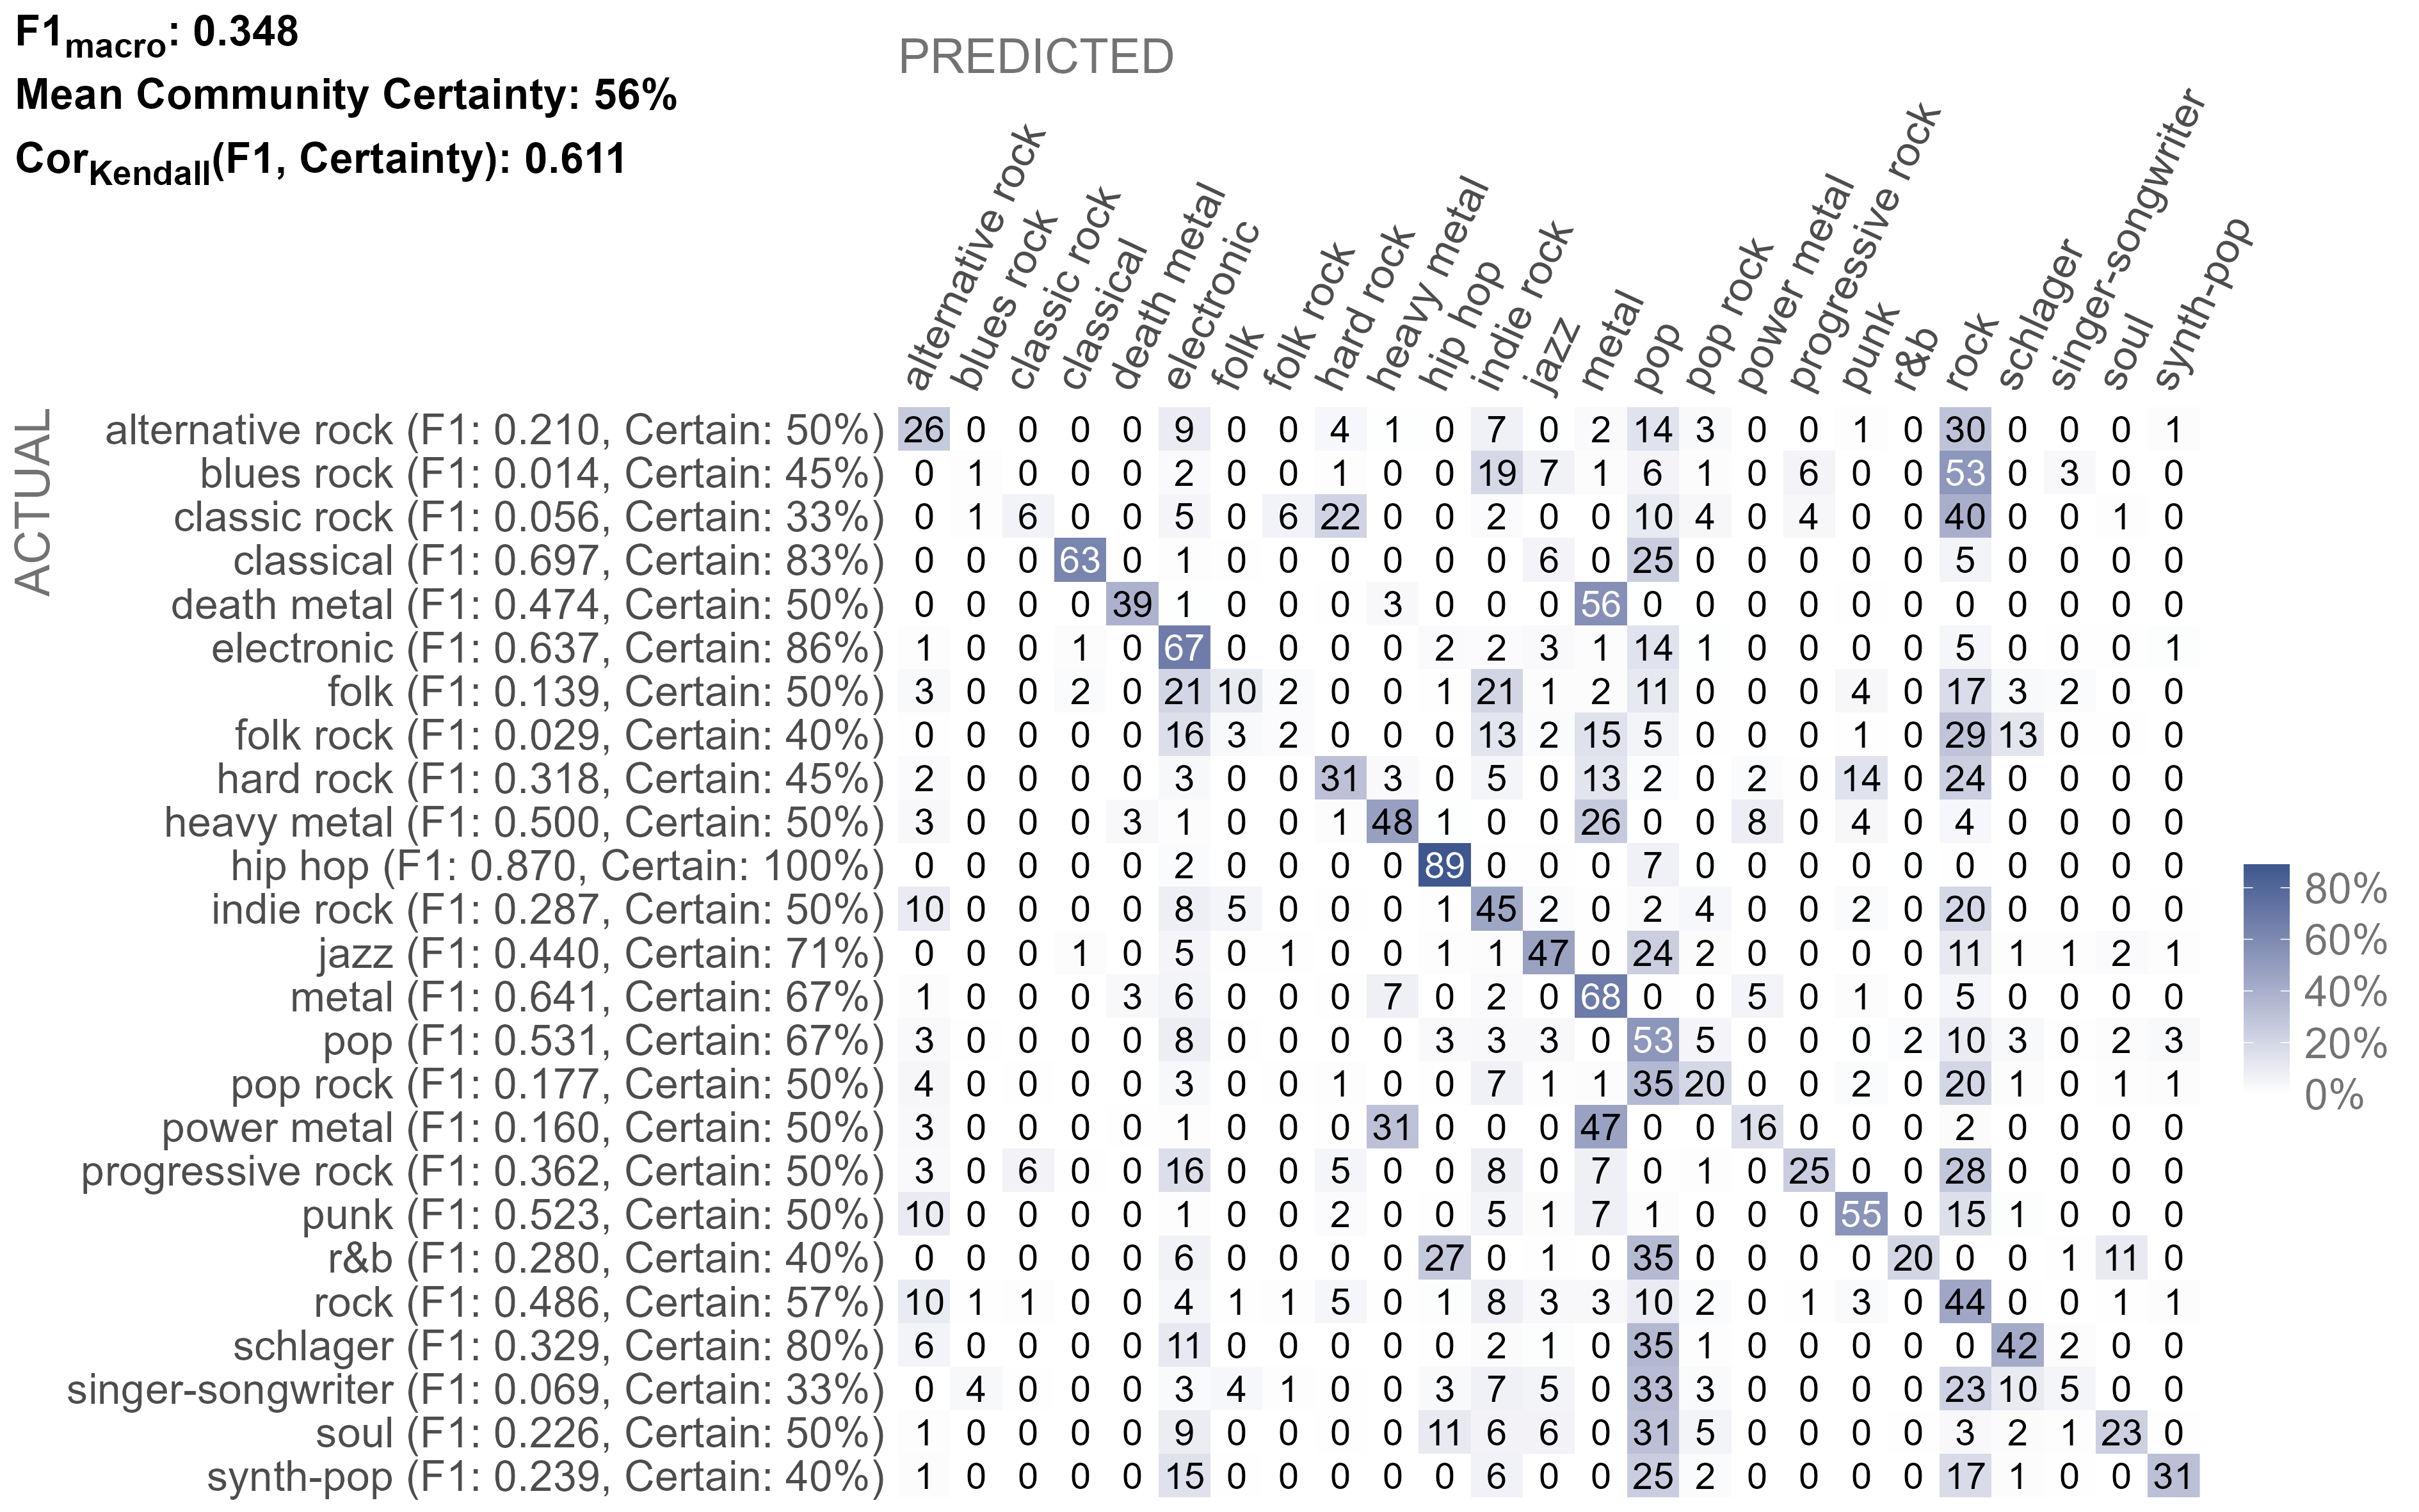
\includegraphics[width=\linewidth]{figures/lightgbm_highres_cm.png}
    \caption{COMGET-G25}
  \end{subfigure}
  \hfill
  \vspace{0 cm}
  \begin{subfigure}[b]{\textwidth}
    \centering
    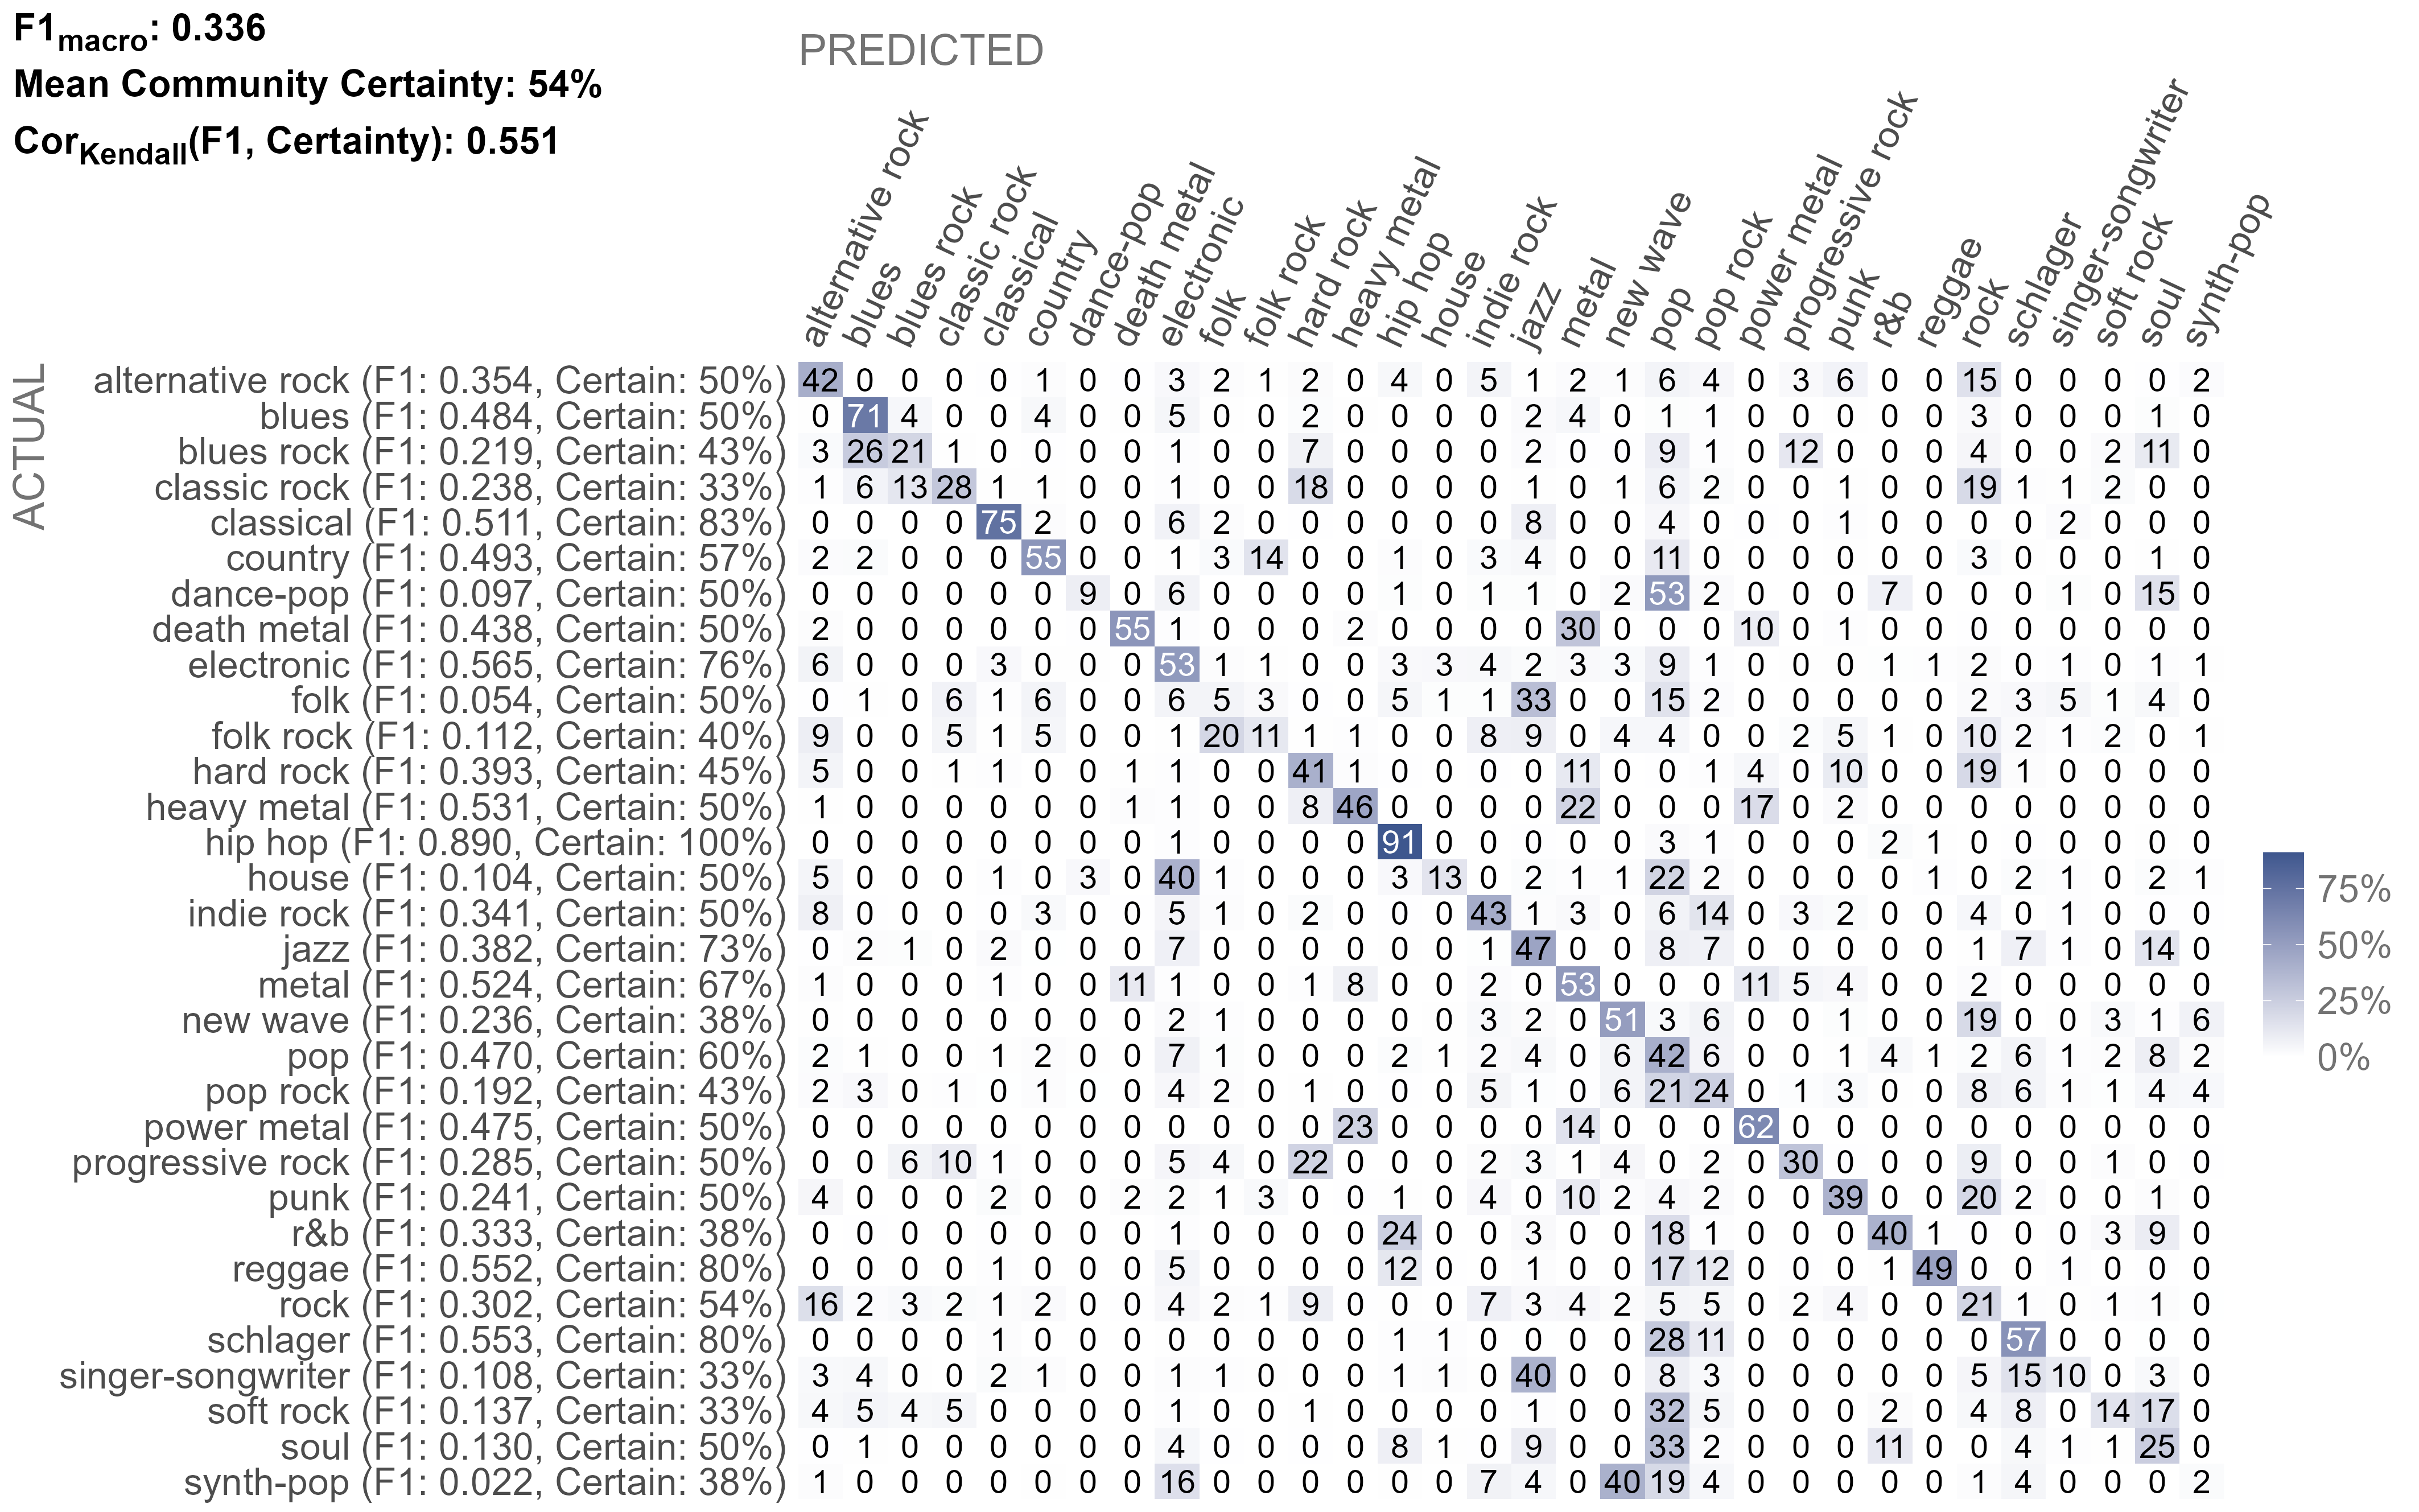
\includegraphics[width=\linewidth]{figures/lightgbm_veryhighres_cm.png}
    \caption{COMGET-G32}
  \end{subfigure}
  \caption{Confusion matrices for the final GBM models on the hold-out set. Values show $P(\text{Predicted}|\text{Actual})$; \textit{certainty} indicates the mean assignment probability for each \textit{genre category} across community votes.}
\label{fig:rq3_appendix_confmat_high_veryhighres}
\end{figure}

\begin{figure}[H]
  \centering
  \begin{subfigure}[b]{\columnwidth}
    \centering
    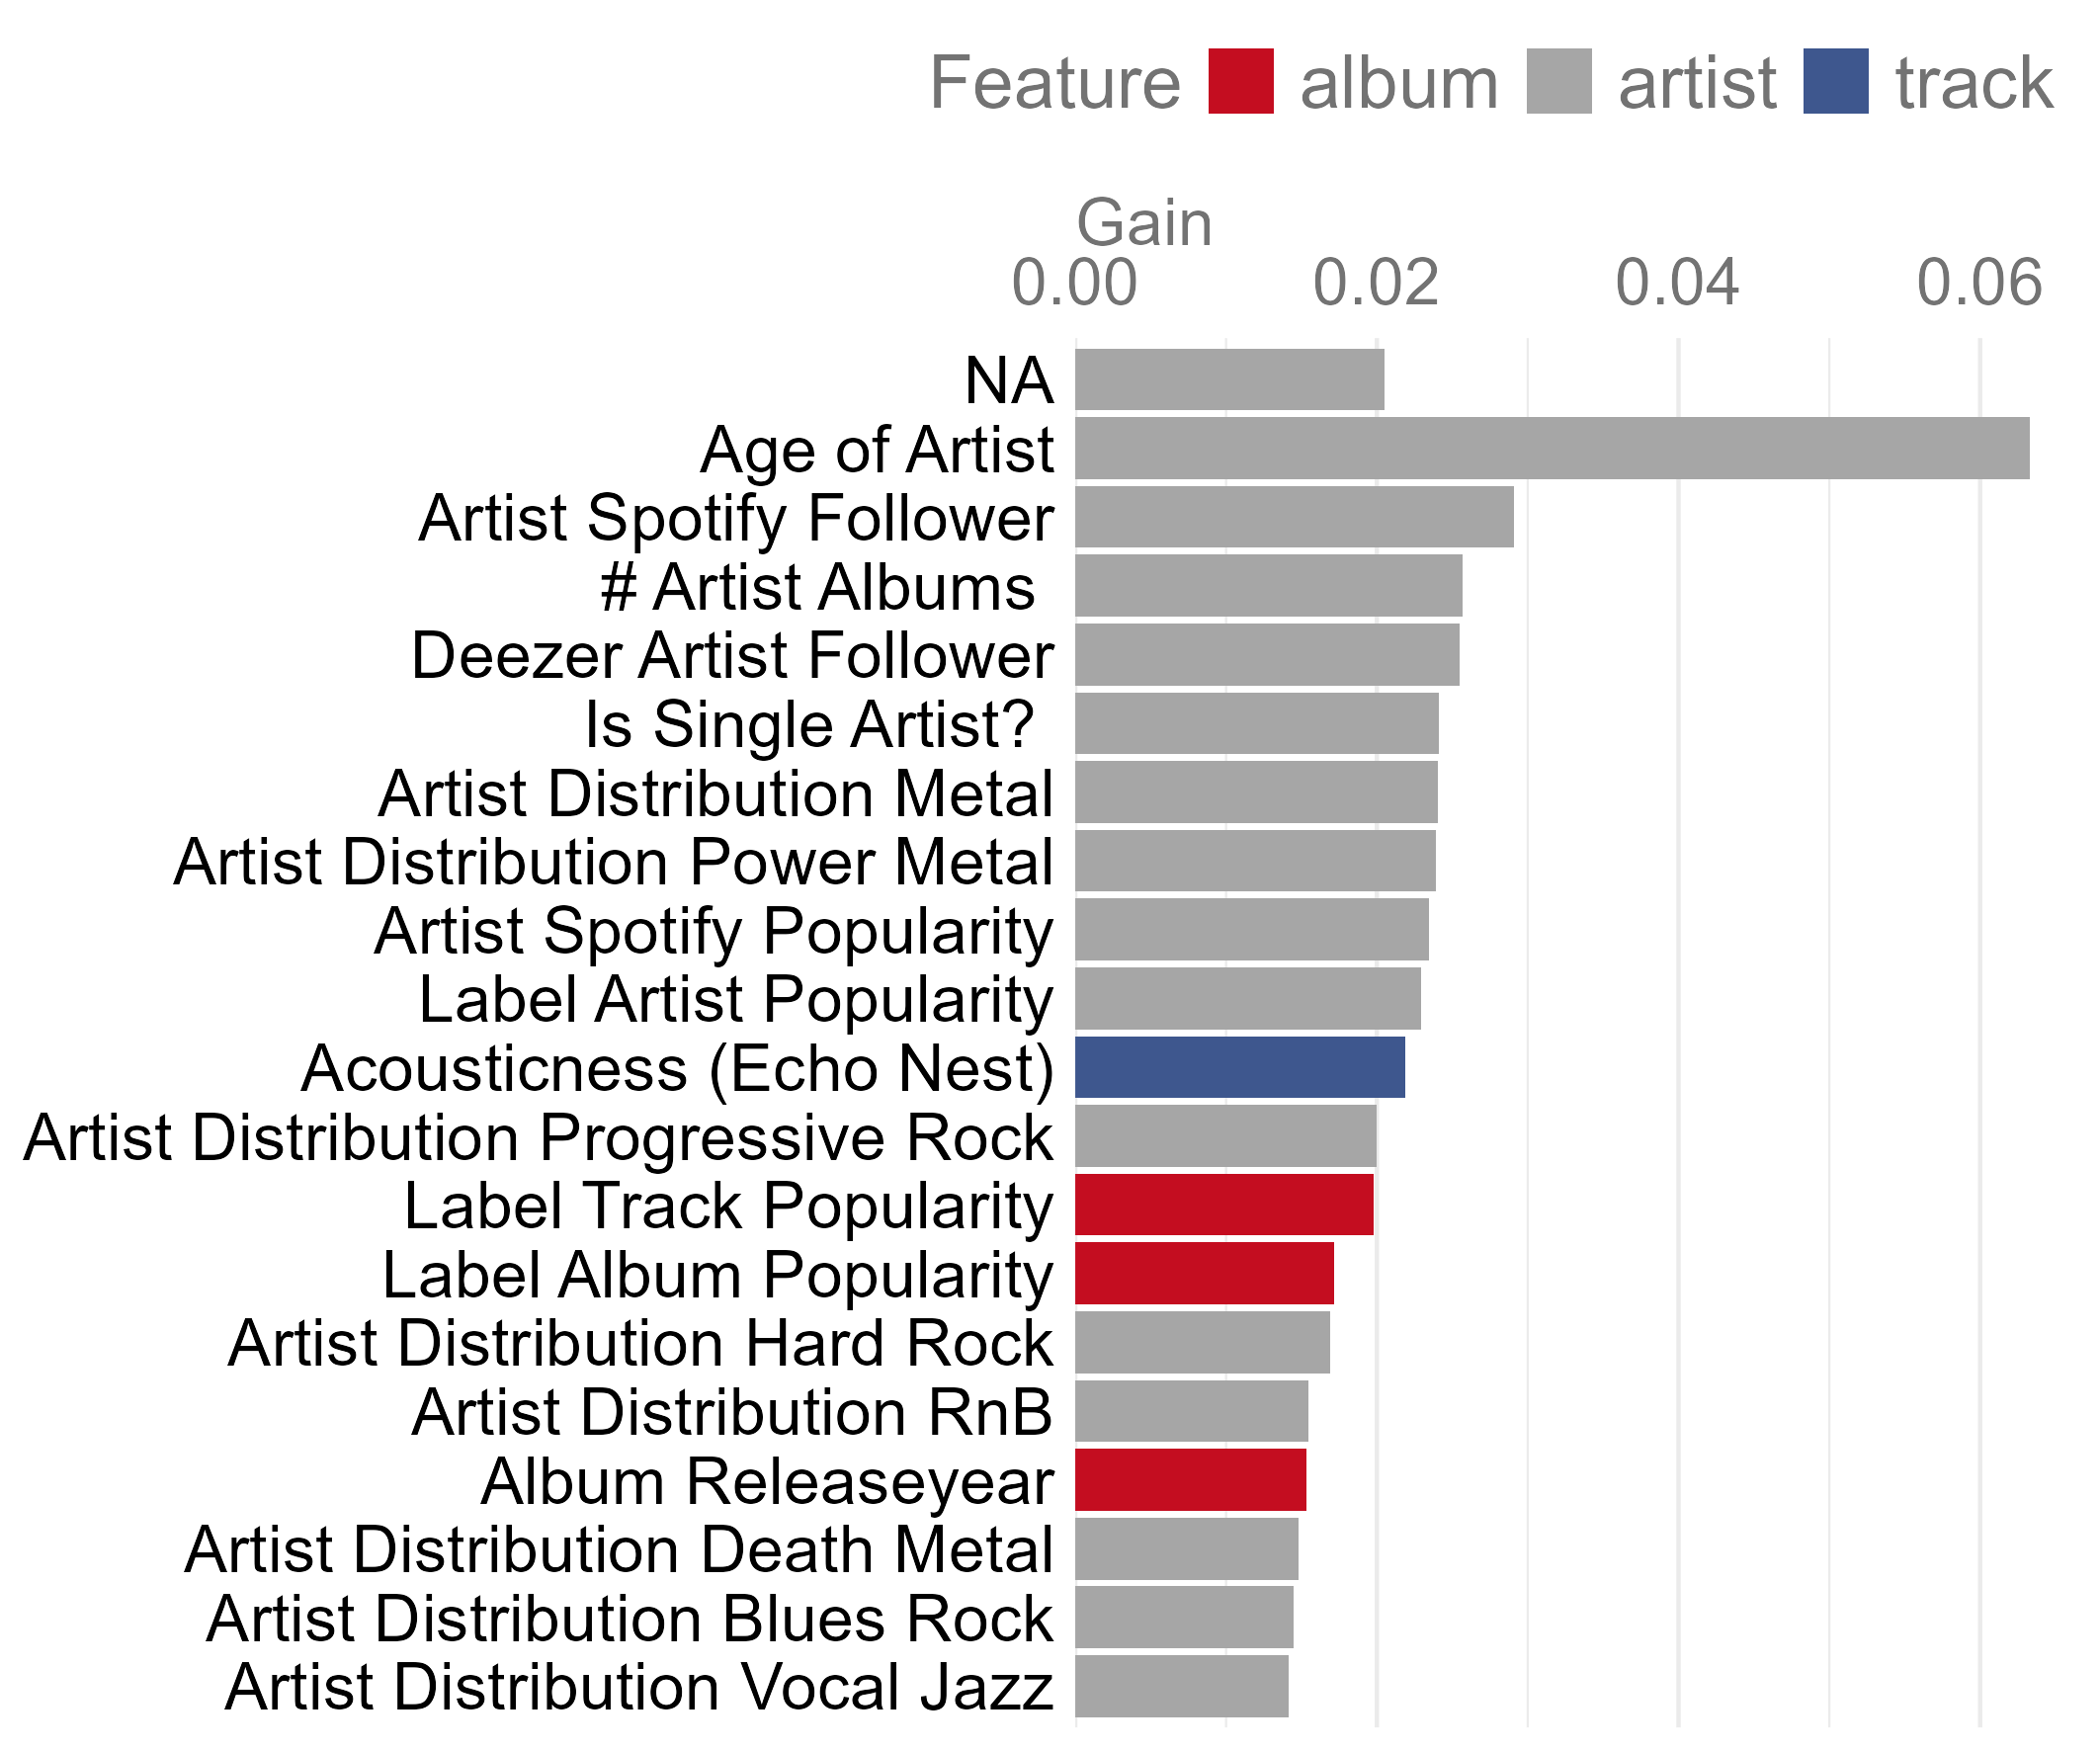
\includegraphics[width=0.6\linewidth]{figures/lightgbm_highres_varimp.png}
    \caption{COMGET-G25}
  \end{subfigure}
  \hfill
  \vspace{0.25 cm}
  \begin{subfigure}[b]{\columnwidth}
    \centering
    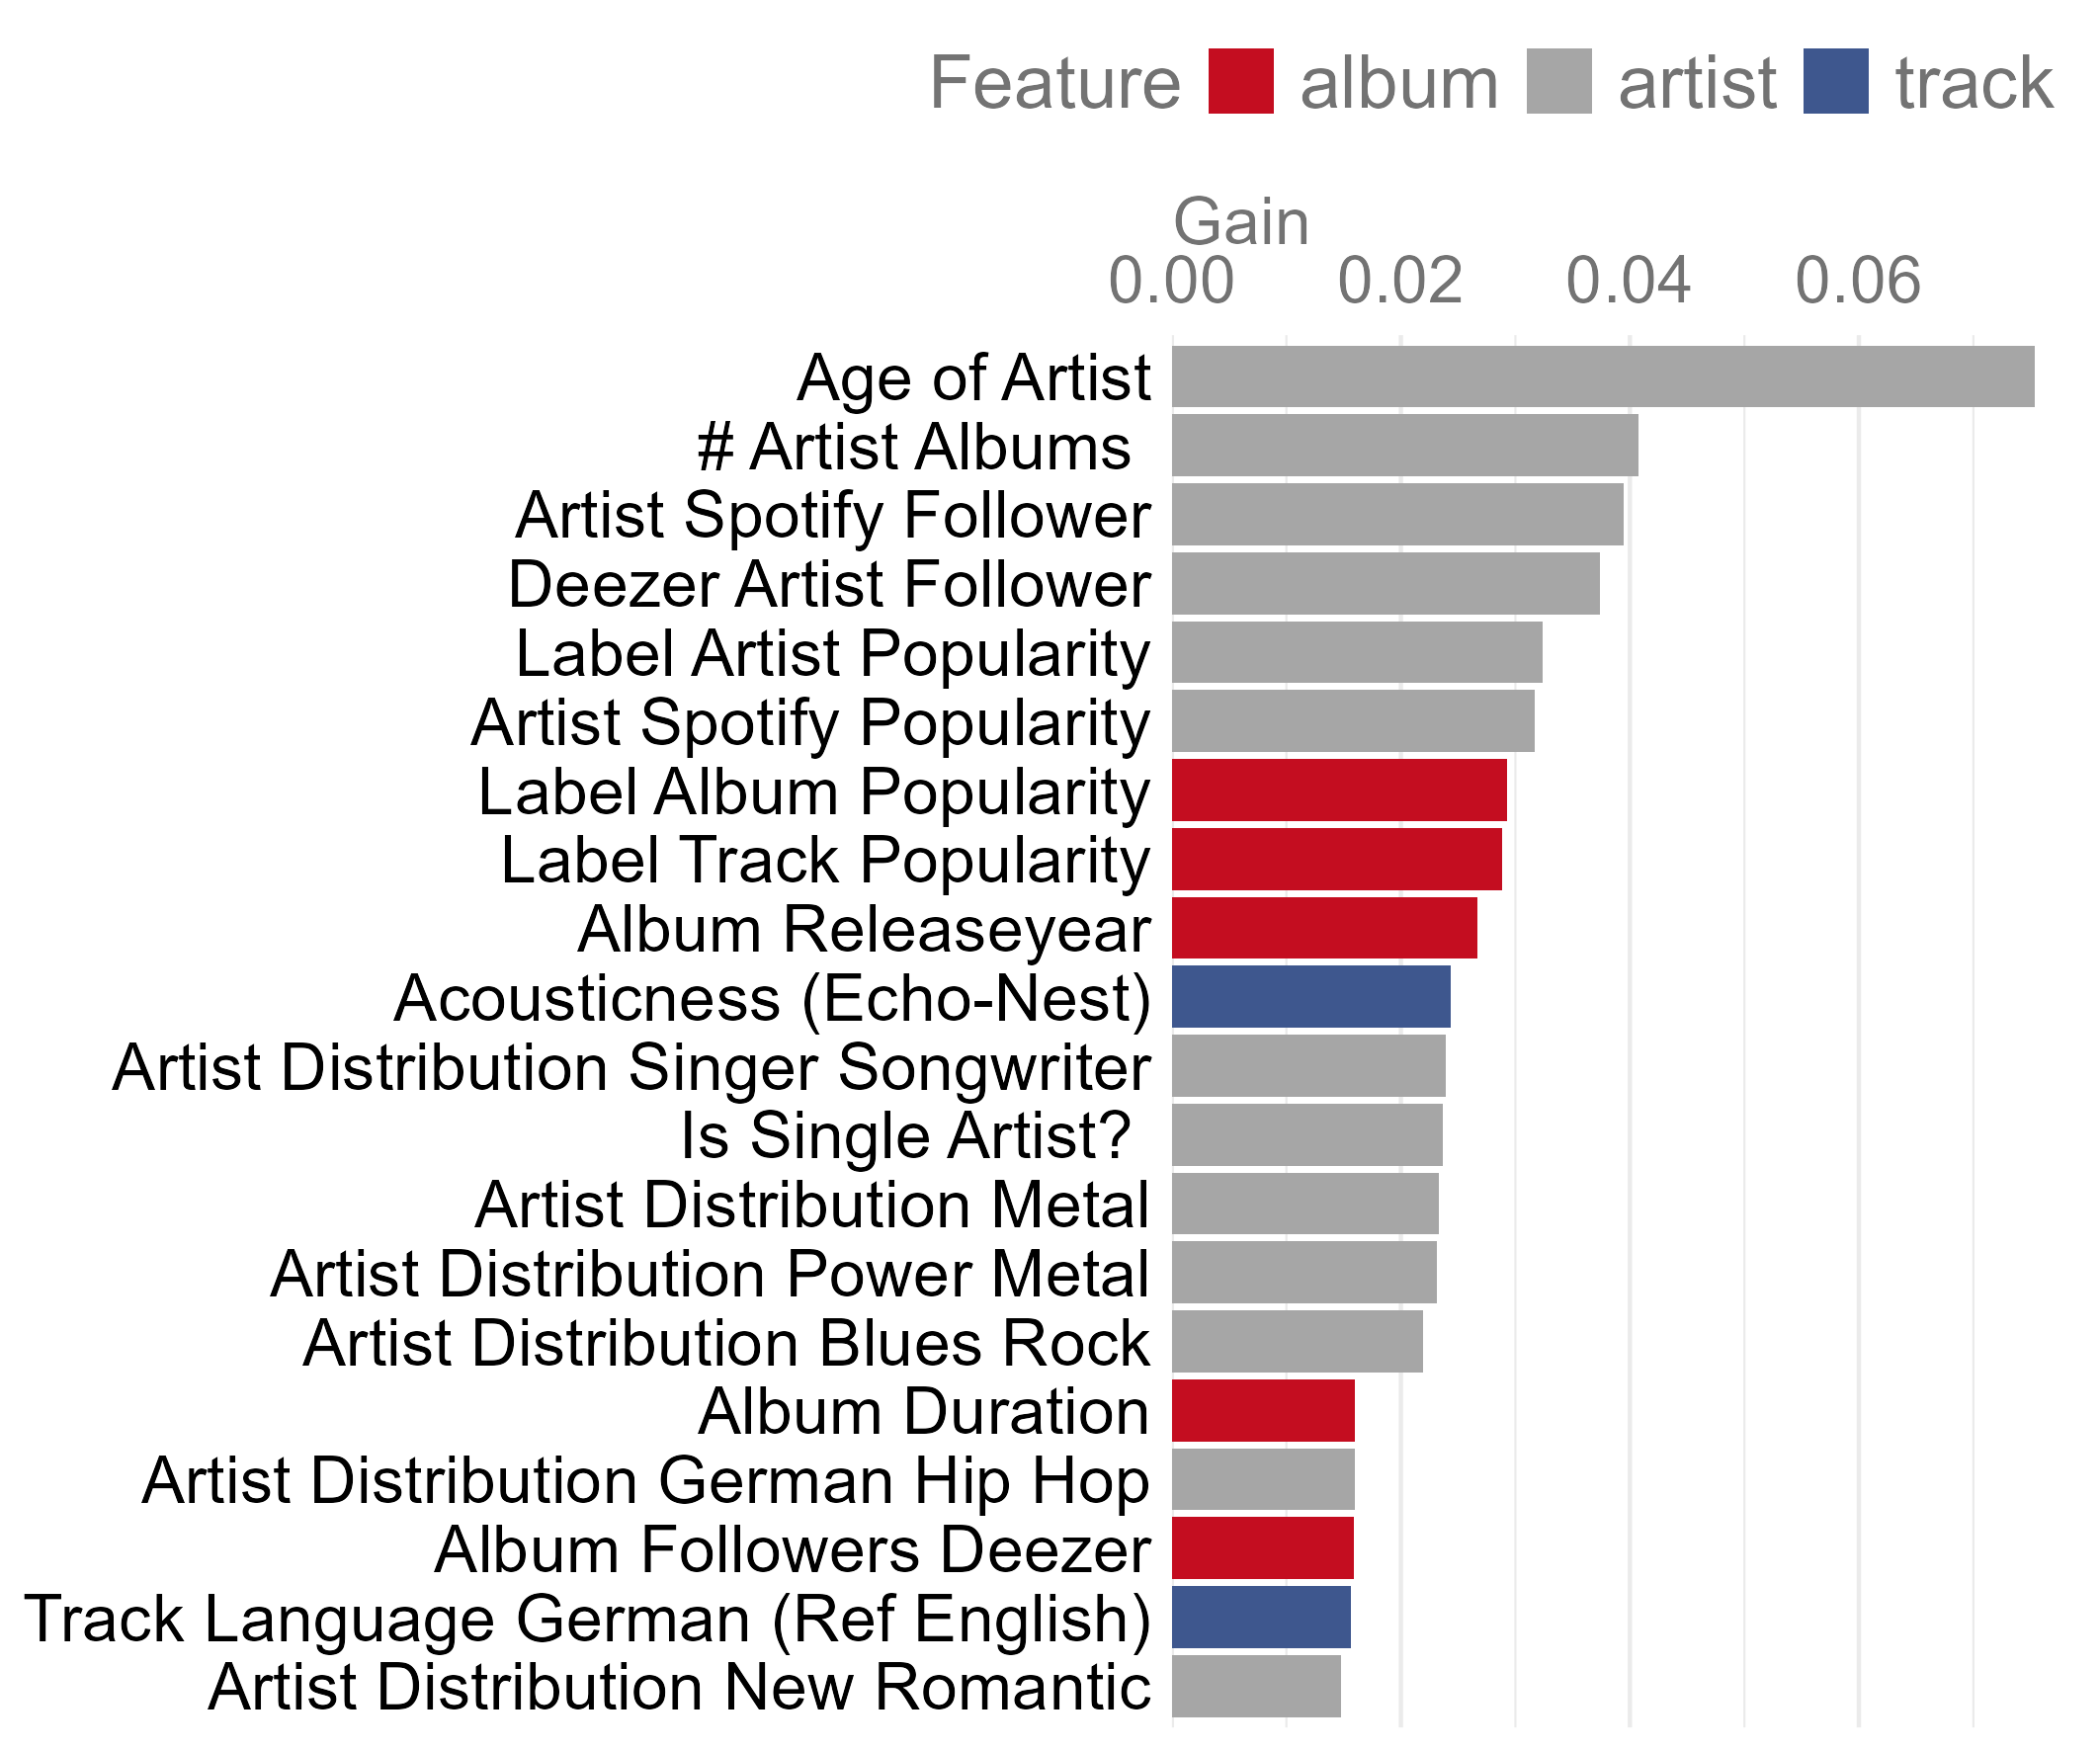
\includegraphics[width=0.6\linewidth, trim={0 0 0 1.5cm}, clip]{figures/lightgbm_veryhighres_varimp.png}
    \caption{COMGET-G32}
  \end{subfigure}
  \caption{Top 20 most important features for automated classification at high and very high granularity. Values show relative feature importance from the final LightGBM models.}
\label{fig:rq3_appendix_varimp_highres_veryhighres}
\end{figure}

\vspace{2cm}
\section{Github Repository}
Please find further details and the complete code for reproduction hosted on \textit{Github}:

\noindent
\textit{Link is left out for the purpose of anonymization of authors}
% \hyperref[https://github.com/markusradke/genrediscourseanalysis]{https://github.com/markusradke/genrediscourseanalysis}%Link would show identify of authors.

\noindent
Data is available from the authors on request.

\end{document}
